We start by describing the details of our experimental platform, the dataset we use, the procedure for generating batches, measuring performance, and then show the results and analysis of our experiments. 



\subsection{Experimental Platform}

For our experiments, we use a system consisting of an NVIDIA Tesla V100 GPU connected to two 48-core CPUs. The Tesla GV100 GPU has 14 TFLOPs of peak single-precision performance, 32 GB/s PCIe bandwidth, and 900 GB/s memory bandwidth. It includes 84 symmetric multiprocessors (SMs), each with 64 independent FP, INT cores, a configurable shared memory size of 96 KB per SM, and is connected to four 4 GB HBM2 DRAM. The Intel Xeon Silver 4116 is a 64-bit, 2.10 GHz (base) Server CPU having 48 x86 cores each, 16.5M L3 cache, and supports DDR4 2400MHz memory. The server is running CentOS 7.9. We use GCC version 9.3 and OpenMP version 5.0 to compile with optimization level 3 (-O3). For all experiments we keep simultaneous multi-threading (SMT) disabled. We use CUDA version 11.3 to compile the GPU programs.
% {\bf CPU:} The system used was a Dell PowerEdge R740 Rack server with two Intel Xeon Silver 4116 CPUs @ 2.10GHz, 128GB DIMM DDR4 Synchronous Registered (Buffered) 2666 MHz (8x16GB) DRAM, 16GB NVIDIA Tesla V100 PCIe GPU (GV100GL), and running CentOS Linux release 7.9.2009 (Core). The Intel Xeon Silver 4116 is a 64-bit, 2.10 GHz (base) Server CPU launched in 2017, that comes with 12 x86 cores each (24 threads with hyper-threading), 16.5M L3 cache, and supports DDR4 2400MHz memory. We use C++ and OpenMP to program our algorithms and the GCC 9 compiler with optimization level 3 (-O3).
% {\bf GPU:} We use an NVIDIA Tesla GV100 (Volta) GPU for our experiments on a GPU. The Tesla GV100 GPU has 14 TFLOPs of peak single-precision performance, 32 GB/s PCIe bandwidth, and 900 GB/s memory bandwidth. It includes 84 SMs, each with 64 independent FP, INT cores, a configurable shared memory size of 96 KB per SM, and is connected to four 4 GB HBM2 DRAM. Volta also supports write-caching (not just load, as previous architectures). Its Address Translation Service (ATS) allows it to access CPU page tables directly (malloc ptr). Its new copy engine does not need pinned memory. Volta's per-thread program-counter, call-stack, allows interleaved executions of warp threads, enabling fine-grained synchronization between threads within a warp. Cooperative groups enable synchronization between warps, grid-wide, multi-GPUs, cross-warp, sub-warp.




\subsection{Dataset}

The graphs we use in our experiments are shown in Table \ref{tab:dataset}. All of them are obtained from the SuiteSparse Matrix Collection \cite{suite19}. For each graph, Table \ref{tab:dataset} lists properties of these graphs including the number of SCCs and the number of levels in the corresponding block-graph. We add self-loops to dead ends in all the graphs. The total number of vertices in the graphs vary from $75$ thousand to $41$  million, and the total number of edges vary from $524$ thousand to $1.1$ billion.

\begin{table}[!hbtp]
\centering
\begin{tabular}{||c||c|c|c|c||}
 \hline
 \textbf{Graph} &
 \textbf{$|V|$} &
 \textbf{$|E|$} &
 \textbf{$SCCs$} &
 \textbf{$Levels$} \\ \hline
 \multicolumn{5}{|c|}{Web Graphs} \\ \hline
  arabic-2005 & 22.7M & 640.0M & 4.0M & 286 \\ \hline
  uk-2005 & 39.5M & 936.4M & 5.8M & 425 \\ \hline
  it-2004 & 41.3M & 1.2B & 6.8M & 278 \\ \hline
  \multicolumn{5}{|c|}{Social Networks} \\ \hline
  soc-Epinions1 & 75.9K & 524.4K & 42.2K & 10 \\ \hline
  soc-LiveJournal1 & 4.8M & 69.5M & 971.2K & 24 \\ \hline
  wiki-Talk & 2.4M & 7.3M & 2.3M & 8 \\ \hline
  \multicolumn{5}{|c|}{Citation/Collaboration Networks} \\ \hline
  cit-Patents & 3.8M & 18.2M & 3.8M & 32 \\ \hline
  coPapersDBLP & 540.5K & 30.5M & 1 & 1 \\ \hline
  amazon-2008 & 735.3K & 5.2M & 90.7K & 6 \\ \hline
  \multicolumn{5}{|c|}{Road/Control-flow Networks} \\ \hline
  italy\_osm & 6.7M & 14.0M & 1 & 1 \\ \hline
  Linux\_call\_graph & 324.1K & 1.3M & 320.1K & 70 \\ \hline
\end{tabular}
\vspace{0.3 cm}
\caption{List of 11 graphs used in our the experiments. Here, $|V|$ is the total number of vertices, $|E|$ is the total number of edges, $SCCs$ is the number of strongly connected components, and $Levels$ is the SCC levels of each fixed graph. The number of vertices and edges are rounded to the nearest thousand (K) or million (M), as appropriate.}
\label{tab:dataset}
\end{table}





\subsection{Batch generation}

We take a base (fixed) graph and generate a batch consisting of random edges to be deleted and inserted. Each batch consists of edge insertions and deletions in an equal mix, and we ensure that no new vertices are added or removed from the graph. The edges to be inserted or deleted are randomly generated, such that edges connecting vertices with high out-degrees have a greater chance of selection. This is done in order to mimic the behaviour of real-world dynamic graphs.
% how performance of each approach is measured, how batches are generated, and then follow up with the details of the specific experiments.

\begin{figure*}[!hbtp]
  \centering

  \subfloat{
    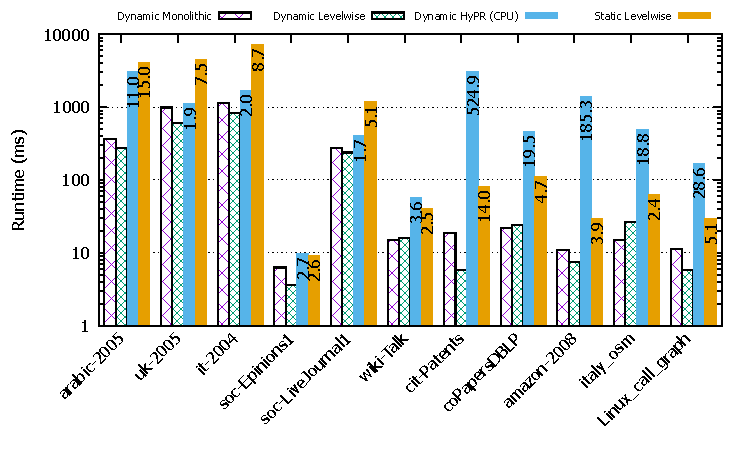
\includegraphics[width=0.48\textwidth]{out/time-omp-am.pdf}
    \label{fig:time-omp-am}
  }
  \subfloat{
    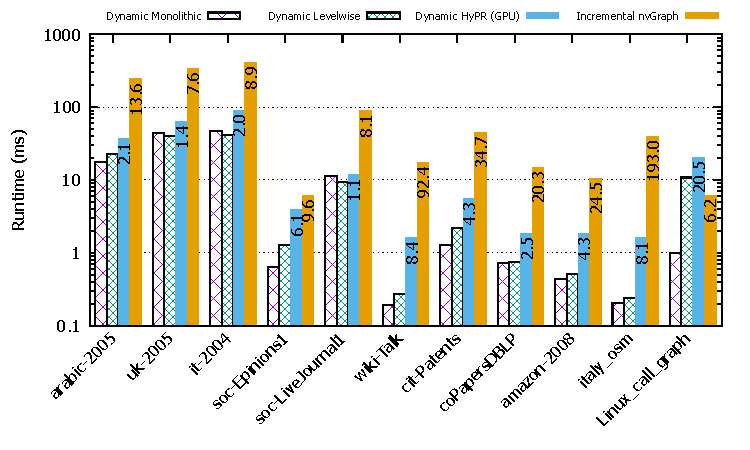
\includegraphics[width=0.48\textwidth]{out/time-cuda-am.pdf}
    \label{fig:time-cuda-am}
  }

  \caption{Time taken for PageRank computation with  \monolithicPR{} and \levelwisePR{} for various batch sizes on the CPU (shown on the left) and the GPU (shown on the right). Batch sizes of 500, 1000, 2000, 5000, and 10000 are used. Time taken with \emph{pure CPU implementation of HyPR} and \emph{plain STIC-D PageRank (static Levelwise)} on the CPU, and speedup of \levelwisePR{} over the two approaches (labeled on top of the respective bars) is also included for comparison. Time taken with \emph{pure GPU implementation of HyPR} and \emph{incremental nvGraph PageRank} on the GPU, and speedup of \monolithicPR{} over the two approaches is included as well.}
  \label{fig:time-am}
\end{figure*}





\subsection{Performance measurement}

We ensure that all the approaches for PageRank computation compared here use the same set of parameters, data types, and other factors determining the time required for computation. We also list out any differences that are beyond our control.

PageRank computation with each approach is performed with a damping factor $d$ of $0.15$, a tolerance $\tau$ of $10^{-6}$, and with a maximum of $500$ iterations. $32-bit$ integers are used for CSR representation, and $32-bit$ floating point values are used for representing ranks for all the approaches. \monolithicPR{} and \levelwisePR{}, along with plain STIC-D PageRank (static Levelwise) use $L\infty{}-norm$ for obtaining the error between the ranks of previous and current iterations. It should however be noted that nvGraph PageRank uses $L2{}-norm$ for error measurement \cite{pr-nvgraph}, which has been observed to converge slower than $L\infty{}-norm$ \cite{gh-levl21}. The measured time in all cases is the rank computation time, and does not include time required to calculate error for convergence check, prepare CSR representation, find affected SCCs, partition vertices by in-degree, group vertices by SCCs, launch kernel (driver overhead), allocate memory, or copy memory between the host (CPU) and the device (GPU). The reported time is the average of multiple runs of respective algorithms. In order to filter out random events affecting the time taken for PageRank computation, each approach is run 5 times and averaged.




\subsection{Results}

\subsubsection{\bf Comparison to Static/Naive Dynamic Approaches}

In this experiment, we compare the performance of \monolithicPR{} (Algorithm \ref{alg:monolithic}) and \levelwisePR{} (Algorithm \ref{alg:levelwise}) with state-of-the-art approaches. In particular, we compare our multicore implementations with the plain STIC-D algorithm (static Levelwise) \cite{pr-sticd16}, which is a static algorithm in the sense that they perform a full recomputation on the new graph. We compare our GPU implementations with the naive dynamic version of nvGraph library implementation of PageRank on a GPU \cite{pr-nvgraph}, a simplified dynamic algorithm which does not skip processing of unaffected vertices (nvGraph does not provide any parameter to control the number of vertices to be processed).
% To the best of our knowledge, there are no dynamic parallel PageRank algorithms to compare our algorithms against. We now describe our experimental results.

\begin{figure*}[!hbtp]
  \centering
  \begin{tikzpicture}
    \draw (0, 0) node[inner sep=0] {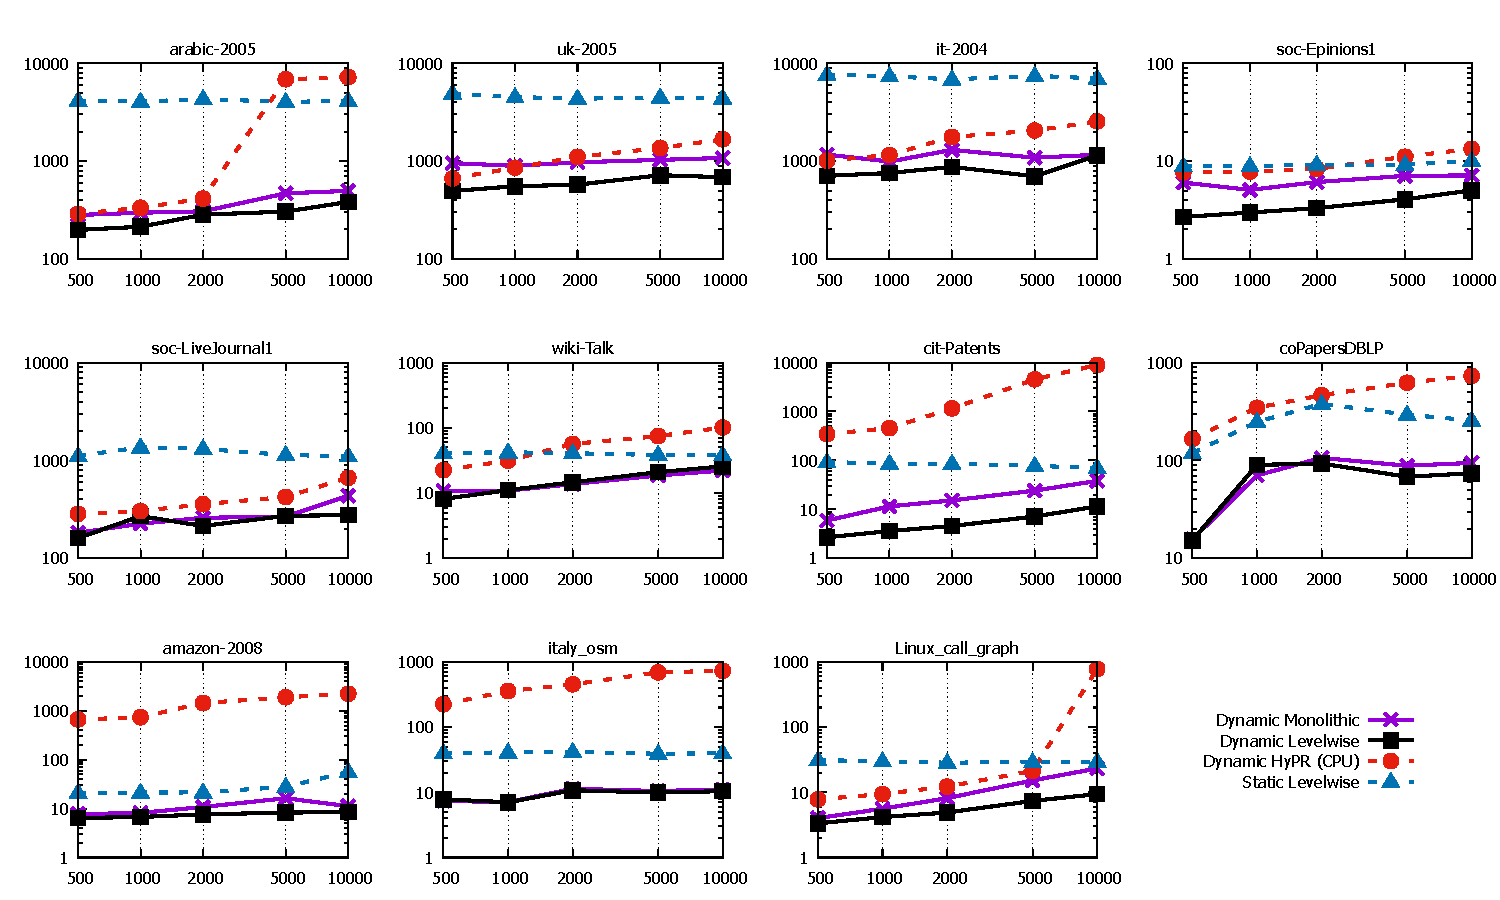
\includegraphics[width=1.00\textwidth]{out/time-omp-all.pdf}};
    \draw (-9.1, 0) node {\rotatebox[origin=t]{90}{Runtime (ms)}};
    \draw (0, -5.7) node {\rotatebox[origin=t]{0}{Batch size}};
  \end{tikzpicture}
  \caption{Time taken for PageRank computation using \monolithicPR{} and \levelwisePR{} on the CPU. Batch sizes of 500, 1000, 2000, 5000, and 10000 are used. Time taken with \emph{pure CPU implementation of HyPR} and \emph{plain STIC-D PageRank (static Levelwise)} is also included for comparison.}
  \label{fig:time-omp-all}
\end{figure*}

\begin{figure*}[!hbtp]
  \centering
  \begin{tikzpicture}
    \draw (0, 0) node[inner sep=0] {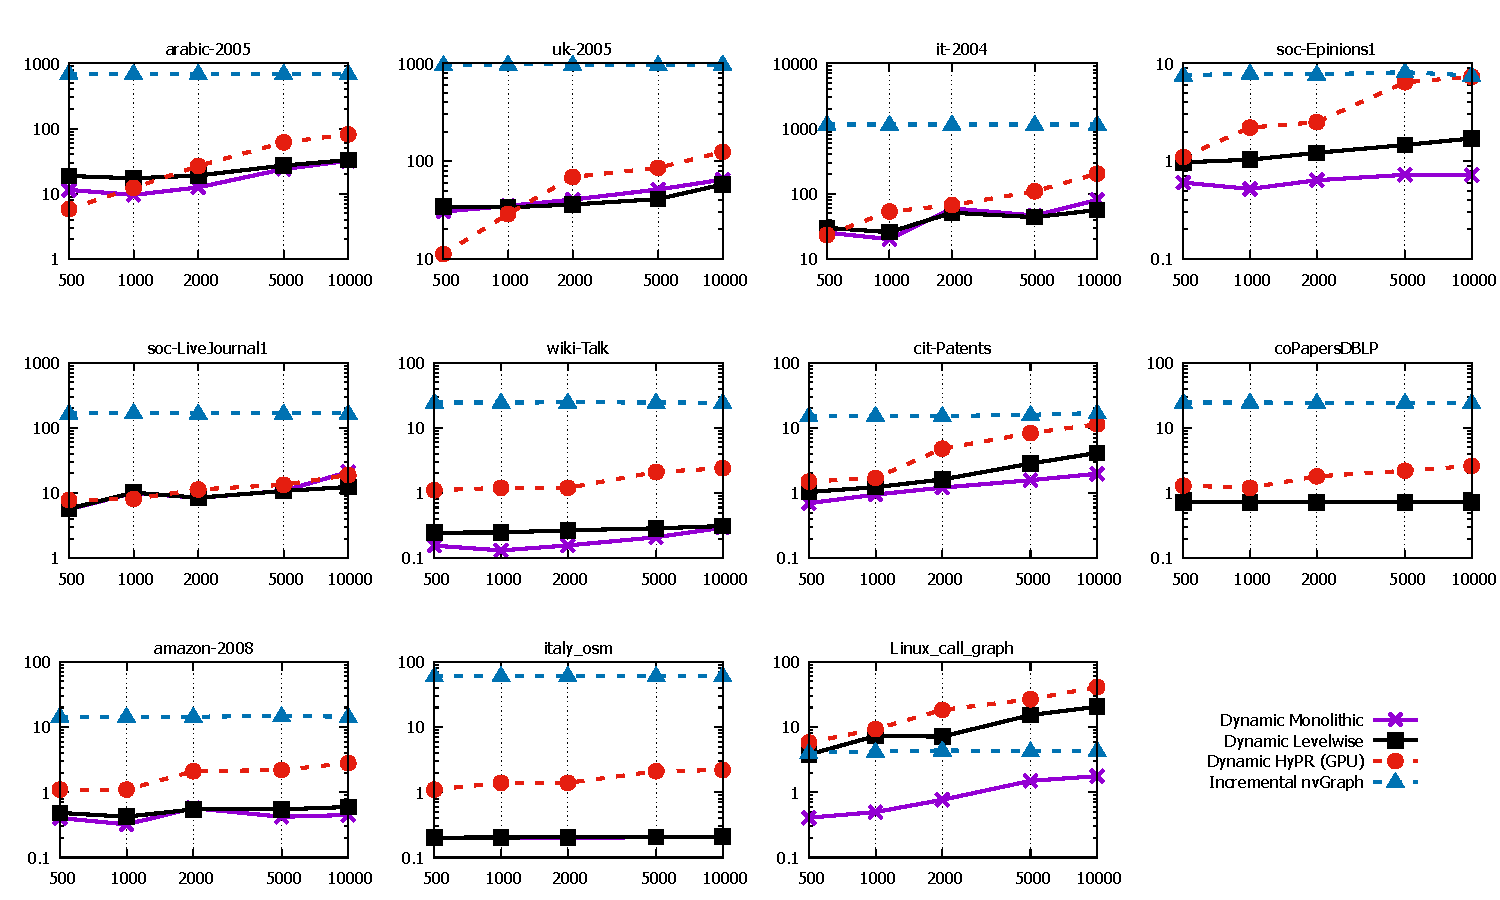
\includegraphics[width=1.00\textwidth]{out/time-cuda-all.pdf}};
    \draw (-9.1, 0) node {\rotatebox[origin=t]{90}{Runtime (ms)}};
    \draw (0, -5.7) node {\rotatebox[origin=t]{0}{Batch size}};
  \end{tikzpicture}
  \caption{Time taken for PageRank computation  using \monolithicPR{} and \levelwisePR{} on the GPU. Batch sizes of 500, 1000, 2000, 5000, and 10000 are used. Time taken with \emph{pure GPU implementation of HyPR} and \emph{incremental nvGraph PageRank} is also included for comparison.}
  \label{fig:time-cuda-all}
\end{figure*}


We experiment with batch sizes of 500, 1000, 2000, 5000, and 10000 edges. The results of this experiment on both the CPU and the GPU is shown in Figure \ref{fig:time-am}. As can be noted from these figures, on the CPU, \monolithicPR{} and \levelwisePR{} achieve an average speedup of 6.1\x and 8.6\x respectively, over the STIC-D algorithm \cite{pr-sticd16}. On the GPU, \monolithicPR{} and \levelwisePR{} achieve an average speedup of 9.8\x and 9.3\x respectively, over the PageRank algorithm from the nvGraph library \cite{pr-nvgraph}. % We observe no significant difference between insertions and deletions and hence the speedup numbers are not reported separately for insertion and deletion batches. 

We observe that \levelwisePR{} performs better on the CPU compared to \monolithicPR{}. \levelwisePR{} is computationally more efficient because it processes SCCs in topological order, avoiding unnecessary recomputation of SCCs that are dependent upon ranks of vertices in other SCCs which have not yet converged. Figure \ref{fig:time-omp-all} shows the detailed run time for each graph and the various batch sizes. We can observe from Figure \ref{fig:time-cuda-all} that \monolithicPR{}{} performs better on the GPU compared to \levelwisePR{}. This is likely due to the presence of levels with insufficient work to keep the GPU busy.

On graphs with a single SCC, viz. {\tt coPapersDBLP} and {\tt italy\_osm} from Table \ref{tab:dataset}, the performance of \levelwisePR{} is almost indistinguishable from \monolithicPR{}. As a single SCC implies a single level in the block graph for \levelwisePR{} to process, its behaviour is identical to that of \monolithicPR{}.




\subsubsection{\bf Comparison to Improved Dynamic approaches}

In this experiment, we compare the performance of the proposed algorithms \monolithicPR{} and \levelwisePR{} with HyPR \cite{hipc19}, a state-of-the-art dynamic PageRank algorithm that only recomputes ranks of affected vertices in the graph. The algorithm from \cite{hipc19} runs in heterogeneous mode and utilizes both the CPU and the GPU simultaneously. To keep our comparison fair, we modify the source code of HyPR to exclusively run either on a CPU or a GPU. We run all the algorithms on a similar set of batches as above.

As seen in Figure \ref{fig:time-am}, we observe a mean speedup of {4.2\x} and {5.8\x} for algorithms \monolithicPR{} and \levelwisePR{} respectively on the CPU, over a pure CPU implementation of HyPR. On the GPU, we observe a mean speedup of {1.9\x} and {1.8\x} for algorithms \monolithicPR{} and \levelwisePR{} respectively, over a pure GPU implementation of HyPR. We also list the detailed run times for each of the approaches with varying batch size on the CPU in Figure \ref{fig:time-omp-all}, and on the GPU in Figure \ref{fig:time-cuda-all}. The speedups can be attributed to grouping of vertices by SCCs and partitioning by in-degree in case of \monolithicPR{}, and due to the processing of affected SCCs in topological ordering in case of \levelwisePR{}.
% of the affected components significantly reduces the amount of work required. This is in contrast to \monolithicPR{} where the work is determined by the affected vertices which incurs significantly higher number of re-computations.
% The performance of HyPR on the GPU seems to approximately proportional to the total number edges, $|E|$. HyPR seems to perform well on web graphs with smaller batch sizes. Why is this? Why it doesn't do th same for larger batch sizes. 
% \kk{this should be comparison to HiPC 2019 paper. The other details are included in the prior subsubsections.}




\subsubsection{\bf Comparison to Single-edge Update}

In this experiment, we study the advantage offered by a batch updates on our algorithms. We take each graph as mentioned in Table \ref{tab:dataset} as the base, and generate a graph delta consisting of a set 10000 edge insertions and deletions, as described in the batch generation section. This graph delta is cumulatively added to the base graph in batches of size 500, 1000, 2000, 5000, and 10000 until the entire graph delta is updated onto the given graph. Each batch, which is a subset of the graph delta, also consists of an equal mix of edge insertions and deletions. After each cumulative update to the graph for the given batch size, PageRank computation is performed with both the dynamic algorithms proposed in this paper, i.e., Algorithms \ref{alg:monolithic} and \ref{alg:levelwise}. Initial ranks are obtained from the ranks of vertices in the previous graph snapshot, as shown in Algorithm \ref{alg:adjust-ranks}. For each approach and batch size combination, the PageRank computation times are measured and summed up. This gives us the total time required for dynamic PageRank computation for a given graph delta, with each approach and batch size combination.

Similar to the process mentioned above, a cumulative single-edge update is performed with the same graph delta upon the base graph, such that edge insertions and deletions alternate with each update. After each update PageRank computation is performed with both the approaches, we obtain the total time needed for the cumulative update by summing up the computation times for each approach. This experiment is performed both on the CPU as well as the GPU.

We observe that a batch update of 5000 edges offers a speedup of {4066\x} and {2998\x} for algorithms \monolithicPR{} and \levelwisePR{} respectively on the CPU, and a speedup of {1712\x} and {2324\x} respectively on the GPU. We show the detailed speedup numbers of  \monolithicPR{} and \levelwisePR{} on each of the 11 input graphs for both the CPU and the GPU in Figure \ref{fig:batch-all}.

From the speedup values, it can be seen that each single-edge update (on average) is only somewhat less expensive than the entire batch update. This seems to suggest that most single-edge updates end up affecting a large number of vertices. This is likely to be the case since batches of edges are generated such that high degree vertices have a higher probability of being changed.

\begin{figure*}[!hbtp]
  \centering

  \subfloat{
    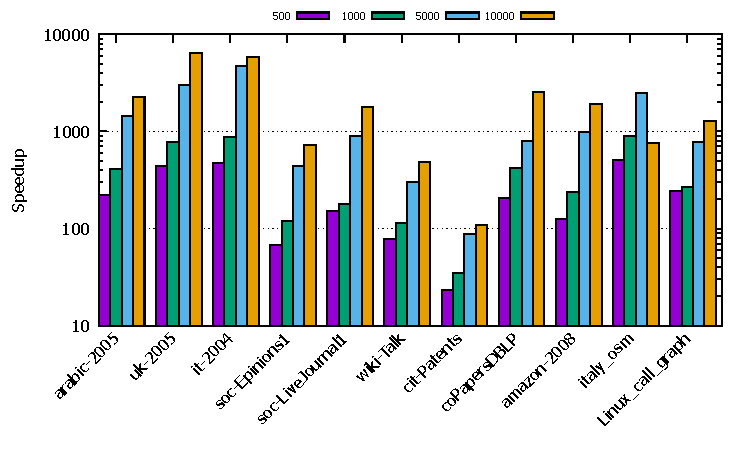
\includegraphics[width=0.48\textwidth]{out/batch-levlomp-all.pdf}
    \label{fig:batch-levlomp-am}
  }
  \subfloat{
    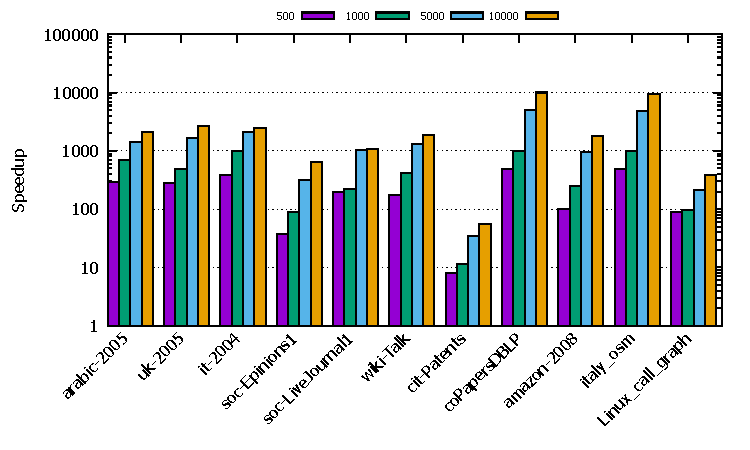
\includegraphics[width=0.48\textwidth]{out/batch-monocuda-all.pdf}
    \label{fig:batch-monocuda-am}
  }

  \caption{Speedup of batched \levelwisePR{} algorithm with respect to cumulative single-edge updates with the same approach on the CPU is shown on the left. Speedup of batched \monolithicPR{} algorithm with respect to cumulative single-edge updates with the same approach on the GPU is shown on the right. Batch sizes of 500, 1000, 5000, and 10000 are shown.}
  \label{fig:batch-all}
\end{figure*}





% \subsection{Batch generation}
% In order to mimic the behaviour of dynamic graphs, a base (fixed) graph is taken and a batch consisting of random edges to be deleted and inserted are generated. Each batch consists of edge insertions and deletions in a 50-50 mix, and it is ensured that no new vertices are added or removed from the graph. The edges to be inserted or deleted are randomly generated, such the edges connecting vertices with high out-degrees have a greater chance of selection.


% To perform our experiments, we do the following preprocessing steps. We first obtain the strongly connected components (SCCs) of the graph using the algorithm of Kosaraju \& Sharir \cite{scc-sharir81}. We sort the SCCs in a topological order of vertices in the block graph, where each SCC represents a vertex and each cross-edge between two SCCs represents  an edge. TODO Multiple cross-edges between SCCs  into a single edge on the block-graph. A simple example of this process is shown in figure \ref{fig:levelwise}. As mentioned before, the vertex order obtained after this process dictates the ordering of  vertices in the CSR representation of the graph. We use this ordering  in our PageRank computation. % Unlike Levelwise PageRank, all vertices (components) were processed in each iteration.
% TODO The convergence criteria for \emph{Monolithic} and \emph{Levelwise PageRank}, \emph{convergence} is reached when the \emph{\textbf{L$\infty$-norm}} between the ranks of \su{\emph{all} vertices (all vertices for monolithic, and vertices in the current level for Levelwise)} in the current and previous iterations falls below the \emph{tolerance value}.
% It is however noted that \emph{nvGraph PageRank} uses \emph{L2-norm} for convergence check \cite{pr-nvgraph-l2norm}, which has been observed to converge \emph{slower} than \emph{L$\infty$-norm} \cite{pr-param21}. \emph{\textbf{nvGraph} PageRank} also seems to use a per iteration \emph{L2-norm rank scaling} (such that sum of square of ranks equals 1) followed by an \emph{L1-norm rank scaling} (such that sum of absolute of ranks equals 1) after the \emph{final iteration}.
% For \emph{dynamic PageRank}, ranks of \emph{affected vertices} are considered for the \emph{L$\infty$-norm}. Ranks of vertices from \emph{previous snapshot} of the graph are \emph{adjusted} before being used as \emph{initial ranks}. It involves a simple \emph{scaling} of ranks based \emph{added/removed vertices}, as shown in Algorithm \ref{alg:adjust-ranks}. A \emph{damping factor} of \emph{0.85}, and a \emph{tolerance} of \emph{$10^{-6}$} is used. The maximum number of iterations allowed is \emph{500}. The PageRank computation is performed on a \emph{Compressed Sparse Row (CSR)} representation of the graph. The \emph{execution time} measured for each test case only includes the time required for \emph{PageRank computation}, including \emph{error calculation}. However, the time required to generate the equivalent graph (if needed), find strongly connected components (SCCs) in topological order (for \emph{Levelwise PageRank}), generate CSR, copy back results from CSR, or allocate memory is \emph{not} included.  With dynamic PageRank, ranks are adjusted from initial ranks.
% \begin{algorithm}[!hbtp]
\caption{Calculation of initial ranks for \emph{dynamic PageRank}, given ranks of vertices for \emph{previous snapshot} of the graph $F(V,E)$, and the \emph{current} graph $G(V,E)$.}
\label{alg:adjust-ranks}
\begin{algorithmic}
% \Require{$F$: Previous snapshot of the graph}
% \Require{$G$: Current snapshot of the graph}
% \Require{$prev$: Ranks of vertices in $F$}
\Function{adjustRanks}{$\vars{F}, \vars{G}, \vars{prev}$}
\State $old \gets F.vertices() \cap G.vertices()$
\State $new \gets G.vertices() - F.vertices()$
\Return{$old: prev[old] \times |V(F)|/|V(G)|, new: 1/|V(G)|$}
\EndFunction
\end{algorithmic}
\end{algorithm}



% \subsection{Performance analysis on CPU}
% \subsection{Performance of Algorithms \ref{alg:monolithic} and \ref{alg:levelwise}}
% In this experiment, we  study the performance of Algorithms [dynamic Monolithic PageRank] and \ref{alg:levelwise}. We compare the performance of our algorithms with state-of-the-art approaches. In particular, we compare our multicore implementation with that of the STIC-D algorithm \cite{pr-sticd16} and with that of the nvGraph library implementation of PageRank on a GPU \cite{pr-nvgraph-l2norm}. Both these algorithms are static algorithms, in the sense that they perform a full recomputation on the new graph. To the best of our knowledge, there are no dynamic parallel PageRank algorithms to compare our algorithms against. We now describe our experimental results.
% In our experiment, we prepare batches of edges to be inserted or deleted from the current graph by choosing such edges uniformly at random. We experiment with batch sizes of  500, 1000, 2000, 5000, and 10000 edges. Each batch of edges fully consists of edges being added or edges being deleted (consists of a 50-50 mix of edges being inserted or deleted, and for single-edge updates, consists only of an edge insertion). 
% REWORD A \emph{single-threaded CPU-based implementation} was used with the first experiment for comparing the approaches, and a \emph{switched thread/block-per-vertex CUDA-based (GPU) implementation} was used with the second one.
%The first experiment used a \textbf{single-threaded CPU-based implementation} to compare the difference in performance of \emph{dynamic Monolithic PageRank}, with \emph{dynamic Levelwise PageRank} on \emph{temporal graphs}. With \emph{(dynamic) Levelwise PageRank}, vertices were grouped by \emph{levels}, which consisted of one or more components in each level. The \emph{level} of each component was obtained from its \emph{topological order} in the \emph{block-graph}. Edges were \emph{inserted} to the graph in \emph{batch sizes} of \emph{500}, \emph{1000}, \emph{5000}, and \emph{10000}. For each batch size, \emph{5 different samples} were taken at different points in time, and their \emph{arithmetic mean (AM)} was obtained.
%Execution time was measured using \emph{std::chrono::high\_performance\_timer}, \emph{5 times} for each test case, and averaged. Statistics of each test case was printed to \emph{standard output (stdout)}, and redirected to a \emph{log file}, which was then processed with a \emph{script} to generate a \emph{CSV file}, with each \emph{row} representing the details of a \emph{single test case}. This \emph{CSV file} was imported into \emph{Google Sheets}, and necessary tables were set up with the help of the \emph{FILTER} function to create the \emph{charts}.


% \kk{Subhajit -- write these as speedup numbers. Not percentages. Speedup = algorithm A time/ algorithm B time, with B being our algorithm and A is the one we are comparing to.}
% \su{Done.}
% \kk{Subhajit: Write one paragraph for CPU and one for GPU. The current plan is to have subsections based on experiments, and not based on platforms. A model is given below.}
% \su{Sir what are the name of subsections?}


% The results of this experiment on the CPU are shown in Figure \ref{fig:time-am} [expt-insert]. As can be seen in these figures, on the CPU Algorithm Levelwise PageRank and Algorithm Monolithic PageRank achieve an average speedup of AAA and BBB respectively, over the STIC-D algorithm \cite{pr-sticd16}. We observe no significant difference between insertions and deletions and hence the speedup numbers are not reported separately for insertion and deletion batches. 
% Figure \ref{fig:time-omp-all} shows the detailed run time for each graph and the various batch sizes. We can observe from Figure \ref{fig:time-cuda-all} that Algorithm Levelwise performs better on the CPU compared to Algorithm Monolithic PageRank. 
% The results of this experiment on the GPU are shown in Figure \ref{fig:time-omp-all} [expt-insert]. As can be seen in these figures, on the GPU Algorithm Levelwise PageRank and Algorithm Monolithic PageRank achieve an average speedup of AAA and BBB respectively, over the PageRank algorithm from the nvGraph library \cite{pr-nvgraph-l2norm}. We observe no significant difference between insertions and deletions and hence the speedup numbers are not reported separately for insertion and deletion batches. 
% Figure \ref{fig:time-omp-all} shows the detailed run time for each graph and the various batch sizes. We can observe from Figure \ref{fig:time-cuda-all} that Algorithm Levelwise performs better on the GPU compared to Algorithm Monolithic PageRank. 


% \kk{Subhajit -- Put these numbers in the earlier paragraphs}


% From the results, it was observed that the speedup of \emph{dynamic Levelwise PageRank} ranges from \emph{0.99x} to \emph{6.25x} for \emph{insertions}, and by \emph{0.99x} to \emph{7.14x} for \emph{deletions}, with respect to \emph{Monolithic} approach (with vertices split by components). For \textbf{edge insertions}, the \textbf{AM speedups} \cite{pr-param21} of \emph{dynamic Levelwise PageRank} are \textbf{2.94x}, \textbf{2.5x}, and \textbf{1.67x} for \emph{batch sizes} of \emph{500}, \emph{1000}, and \emph{10000} respectively. For \textbf{edge deletions}, the \textbf{AM speedups} are \textbf{3.45x}, \textbf{3.03x}, and \textbf{2.22x}. Here, \emph{AM speedup} was obtained by taking the \emph{arithmetic mean (AM)} of time taken for PageRank computation for insertions/deletions of a particular batch size on all graphs, and then obtaining a ratio \emph{relative} to the \emph{Monolithic} approach.


%\su{Sir although figures for only 500, 1000, and 10000 batch sizes, i ran the expt. with $10$ to $10^8$ batch sizes. Single edge update is just too small and in many cases would likely complete in no time. KK: Repeat the single edge update over the entire batch size. In essence, if the bath size is 100, you run 100 single edge updates and then run the 1 batch of 100. What is the time difference between these two?}


% \subsection{Performance analysis on GPU}
% The second experiment is similar to the first experiment, except that it uses a \textbf{switched thread/block-per-vertex CUDA-based (GPU) implementation} \cite{pr-volta21}. Additionally, \emph{nvGraph's incremental PageRank} approach was also included for reference. Note that \emph{nvGraph} does \emph{not} support \emph{dynamic PageRank}. With \emph{(dynamic) Monolithic PageRank}, vertices were grouped by \emph{large components}, and \emph{partitioned by in-degree} based on a suitable \emph{switch-point} \cite{pr-volta21}. \emph{Large components} were obtained by \emph{combining} together components until they satisfied a \emph{min-compute} of $10^7$. With \emph{(dynamic) Levelwise PageRank}, vertices were grouped by \emph{levels}, which consisted of one or more components in each level, and \emph{partitioned by in-degree} similarly. Rest of the process was similar to that of the first experiment.
% From the results of the second experiment it was observed that the speedup of \emph{dynamic Levelwise PageRank} ranges from \emph{1.51x} to \emph{0.02x} for \emph{insertions}, and by \emph{0.63x} to \emph{0.02x} for \emph{deletions}, with respect to \emph{Monolithic} approach (with vertices split by components). For \textbf{edge insertions}, the \textbf{AM speedups} between \emph{dynamic Monolithic} and \emph{Levelwise PageRank} is \textbf{0.13x} for all \emph{batch sizes} of \emph{500}, \emph{1000}, and \emph{10000}. For \textbf{edge deletions}, the \textbf{AM-RATIOs} are \textbf{0.12x}, \textbf{0.12x}, and \textbf{0.18x}.


% \paragraph{Discussion:}
% From the results of the first experiment using a \textbf{single-threaded CPU-based implementation}, it can be inferred that the \emph{Levelwise} approach to PageRank computation, on a \emph{CPU}, is \emph{about 20-30\% faster than} the \emph{Monolithic} approach. This seems intuitive as Levelwise PageRank processes components in \emph{topological order}, and convergence of components on \emph{higher levels} of the block-graph \emph{should ideally} help accelerate the convergence of the \emph{lower levels}. It is also possible that this could be due to \emph{faster satisfaction} of \emph{convergence criterion} of \emph{each level} (with Levelwise approach), in contrast to convergence of \emph{all the vertices} (with Monolithic approach). Analysis of convergence rate of components/levels might help in understanding the cause, which may be explored in future work. Indeed, \emph{slightly higher} error, with respect to nvGraph PageRank, is observed with the \emph{Levelwise approach}. However, given the fact that Levelwise PageRank is a suitable technique for \emph{distributed PageRank computation} for \emph{dead ends free graphs}, it is a small price to pay.
% The second experiment, which uses a \textbf{switched thread / block-per-vertex CUDA-based (GPU) implementation}, suggests that \emph{Levelwise PageRank} is \emph{significantly slower} than \emph{Monolithic PageRank}. This overwhelming increase in PageRank computation time is most likely due to the existence of a large number of \emph{small sized levels}, consisting of small components. This would cause a \emph{large number of CUDA kernel calls} to be made for each level, which can in act as a \emph{major bottleneck} on the system. Thus, the vanilla Levelwise approach would be \emph{unsuitable} for use with \emph{GPU} unless measures are taken to \emph{combine smaller levels/components} in order to ensure sufficient workload on the GPU per kernel call.


% \kk{Are we doing additional optimizations? We should then also add these details to the section on algorithmic details and show the impact of these optimizations. This kind of analysis per graph class and per optimization adds a lot of value to the paper.}
% \su{Sir, ICD optimizations have not been included.}


% \subsubsection{Comparison to Single Edge Update}
% \subsection{Results and Discussion}
% List of experiments : Replicate over CPU, GPU, and multi-GPU
% \begin{itemize}
%   \item Comparison wrt single update
%   \item Comparison wrt nvGraph black box, cuGraph modified as STIC-D
%   \item Batch size Vs Performance
%   \item Scalability? 
% \end{itemize}
% * CPU Vs GPU: Compare across CPU and GPU
% * Versions of STIC-D driven algorithms on various graph classes: which feature is more suitable for which graph class
